\documentclass[journal,12pt,twocolumn]{IEEEtran}
%

\def\inputGnumericTable{}
\usepackage{setspace}
\usepackage{gensymb}
%\doublespacing
\singlespacing

%\usepackage{graphicx}
%\usepackage{amssymb}
%\usepackage{relsize}
\usepackage[cmex10]{amsmath}
%\usepackage{amsthm}
%\interdisplaylinepenalty=2500
%\savesymbol{iint}
%\usepackage{txfonts}
%\restoresymbol{TXF}{iint}
%\usepackage{wasysym}
\usepackage{amsthm}
%\usepackage{iithtlc}
\usepackage{mathrsfs}
\usepackage{txfonts}
\usepackage{stfloats}
\usepackage{bm}
\usepackage{cite}
\usepackage{cases}
\usepackage{subfig}
%\usepackage{xtab}
\usepackage{longtable}
\usepackage{multirow}
%\usepackage{algorithm}
%\usepackage{algpseudocode}
\usepackage{enumitem}
\usepackage{mathtools}
\usepackage{steinmetz}
\usepackage{tikz}
\usepackage{circuitikz}
\usepackage{verbatim}
\usepackage{tfrupee}
\usepackage[breaklinks=true]{hyperref}
%\usepackage{stmaryrd}
\usepackage{tkz-euclide} % loads  TikZ and tkz-base
%\usetkzobj{all}
\usetikzlibrary{calc,math}
\usepackage{listings}
    \usepackage{color}                                            %%
    \usepackage{array}                                            %%
    \usepackage{longtable}                                        %%
    \usepackage{calc}                                             %%
    \usepackage{multirow}                                         %%
    \usepackage{hhline}                                           %%
    \usepackage{ifthen}                                           %%
  %optionally (for landscape tables embedded in another document): %%
    \usepackage{lscape}     
\usepackage{multicol}
\usepackage{chngcntr}
%\usepackage{enumerate}

%\usepackage{wasysym}
%\newcounter{MYtempeqncnt}
\DeclareMathOperator*{\Res}{Res}
%\renewcommand{\baselinestretch}{2}
\renewcommand\thesection{\arabic{section}}
\renewcommand\thesubsection{\thesection.\arabic{subsection}}
\renewcommand\thesubsubsection{\thesubsection.\arabic{subsubsection}}

\renewcommand\thesectiondis{\arabic{section}}
\renewcommand\thesubsectiondis{\thesectiondis.\arabic{subsection}}
\renewcommand\thesubsubsectiondis{\thesubsectiondis.\arabic{subsubsection}}

% correct bad hyphenation here
\hyphenation{op-tical net-works semi-conduc-tor}
\def\inputGnumericTable{}                                 %%

\lstset{
%language=C,
frame=single, 
breaklines=true,
columns=fullflexible
}
%\lstset{
%language=tex,
%frame=single, 
%breaklines=true
%}

\begin{document}
%


\newtheorem{theorem}{Theorem}[section]
\newtheorem{problem}{Problem}
\newtheorem{proposition}{Proposition}[section]
\newtheorem{lemma}{Lemma}[section]
\newtheorem{corollary}[theorem]{Corollary}
\newtheorem{example}{Example}[section]
\newtheorem{definition}[problem]{Definition}
%\newtheorem{thm}{Theorem}[section] 
%\newtheorem{defn}[thm]{Definition}
%\newtheorem{algorithm}{Algorithm}[section]
%\newtheorem{cor}{Corollary}
\newcommand{\BEQA}{\begin{eqnarray}}
\newcommand{\EEQA}{\end{eqnarray}}
\newcommand{\define}{\stackrel{\triangle}{=}}
\bibliographystyle{IEEEtran}
%\bibliographystyle{ieeetr}
\providecommand{\mbf}{\mathbf}
\providecommand{\pr}[1]{\ensuremath{\Pr\left(#1\right)}}
\providecommand{\qfunc}[1]{\ensuremath{Q\left(#1\right)}}
\providecommand{\sbrak}[1]{\ensuremath{{}\left[#1\right]}}
\providecommand{\lsbrak}[1]{\ensuremath{{}\left[#1\right.}}
\providecommand{\rsbrak}[1]{\ensuremath{{}\left.#1\right]}}
\providecommand{\brak}[1]{\ensuremath{\left(#1\right)}}
\providecommand{\lbrak}[1]{\ensuremath{\left(#1\right.}}
\providecommand{\rbrak}[1]{\ensuremath{\left.#1\right)}}
\providecommand{\cbrak}[1]{\ensuremath{\left\{#1\right\}}}
\providecommand{\lcbrak}[1]{\ensuremath{\left\{#1\right.}}
\providecommand{\rcbrak}[1]{\ensuremath{\left.#1\right\}}}
\theoremstyle{remark}
\newtheorem{rem}{Remark}
\newcommand{\sgn}{\mathop{\mathrm{sgn}}}
\providecommand{\abs}[1]{\left\vert#1\right\vert}
\providecommand{\res}[1]{\Res\displaylimits_{#1}} 
\providecommand{\norm}[1]{\left\lVert#1\right\rVert}
%\providecommand{\norm}[1]{\lVert#1\rVert}
\providecommand{\mtx}[1]{\mathbf{#1}}
\providecommand{\mean}[1]{E\left[ #1 \right]}
\providecommand{\fourier}{\overset{\mathcal{F}}{ \rightleftharpoons}}
%\providecommand{\hilbert}{\overset{\mathcal{H}}{ \rightleftharpoons}}
\providecommand{\system}{\overset{\mathcal{H}}{ \longleftrightarrow}}
	%\newcommand{\solution}[2]{\textbf{Solution:}{#1}}
\newcommand{\solution}{\noindent \textbf{Solution: }}
\newcommand{\cosec}{\,\text{cosec}\,}
\providecommand{\dec}[2]{\ensuremath{\overset{#1}{\underset{#2}{\gtrless}}}}
\newcommand{\myvec}[1]{\ensuremath{\begin{pmatrix}#1\end{pmatrix}}}
%\newcommand{\myvec}[1]{\ensuremath{\begin{pmatrix}#1\end{pmatrix}}}
\newcommand{\mydet}[1]{\ensuremath{\begin{vmatrix}#1\end{vmatrix}}}
%\numberwithin{equation}{section}
\numberwithin{equation}{subsection}
%\numberwithin{problem}{section}
%\numberwithin{definition}{section}
\makeatletter
\@addtoreset{figure}{problem}
\makeatother
\let\StandardTheFigure\thefigure
\let\vec\mathbf
%\renewcommand{\thefigure}{\theproblem.\arabic{figure}}
%\renewcommand{\thefigure}{\theproblem}
%\setlist[enumerate,1]{before=\renewcommand\theequation{\theenumi.\arabic{equation}}
%\counterwithin{equation}{enumi}
%\renewcommand{\theequation}{\arabic{subsection}.\arabic{equation}}
\def\putbox#1#2#3{\makebox[0in][l]{\makebox[#1][l]{}\raisebox{\baselineskip}[0in][0in]{\raisebox{#2}[0in][0in]{#3}}}}
     \def\rightbox#1{\makebox[0in][r]{#1}}
     \def\centbox#1{\makebox[0in]{#1}}
     \def\topbox#1{\raisebox{-\baselineskip}[0in][0in]{#1}}
     \def\midbox#1{\raisebox{-0.5\baselineskip}[0in][0in]{#1}}
\vspace{3cm}
\title{LinearAlgebra Question 5}
\author{Srihari S}


\maketitle
\begin{abstract}
A document implementing solutions to problems using linear algebra.
\end{abstract}
Download all python codes from 
%
\begin{lstlisting}
svn co https://github.com/Srihari123456/Summer-2020/tree/master/LinearAlgebrafolder/codes
\end{lstlisting}
Download all \LaTeX{}-Tikz codes from 
%
\begin{lstlisting}
svn co https://github.com/Srihari123456/Summer-2020/tree/master/LinearAlgebrafolder/figs
\end{lstlisting}

%\section{\textbf{Question 1.1.5}}
%\subsection{Problem}
\renewcommand{\theequation}{\theenumi}
\begin{enumerate}[label=\thesection.\arabic*.,ref=\thesection.\theenumi]
\numberwithin{equation}{enumi}
\item Find the area of the triangle having vertices 
\begin{multline}
	\vec{A} = \myvec{1\\1\\1}\quad
	\vec{B} = \myvec{1\\2\\3}\quad
	\vec{C} = \myvec{2\\3\\1}
\end{multline}
	The following python code computes the area of $\triangle$ABC in Fig.\ref{fig:qone}.
	\begin{lstlisting}
	./codes/triangle/q1.py
	\end{lstlisting}
	\solution The area of $\triangle$ABC is defined as
	\begin{align}
		\frac{1}{2}\norm{\brak{\vec{B-A}} \times \brak{\vec{C-A}}}
	\end{align}
	\begin{figure}[!ht]
	\centering
	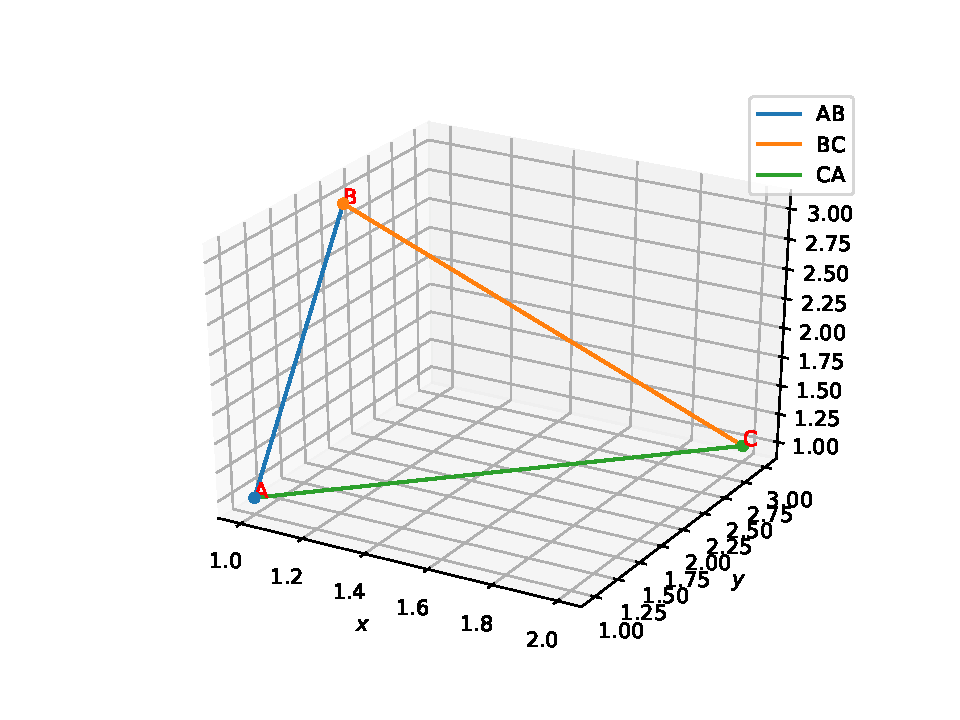
\includegraphics[width=\columnwidth]{./figs/triangle/q1.pdf}
	\caption{Triangle of Q.1.1.5}
	\label{fig:qone}	
	\end{figure}
	which is calculated and found as 2.29
\end{enumerate}


\section{\textbf{Question 1.2.5}}
	The following python code computes the length of the altitude $\vec{AD}$ in Fig.\ref{fig:1.2.5_qtwo}.
	\begin{lstlisting}
	./solutions/5/codes/triangle/q2.py
	\end{lstlisting}
	
	\begin{figure}[!ht]
	\centering
	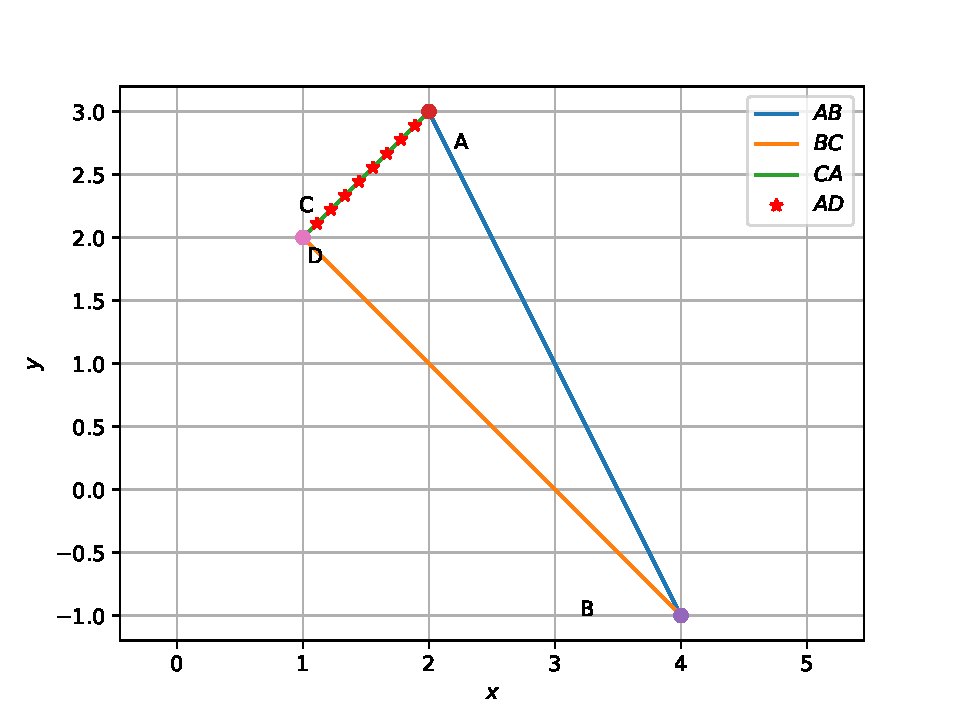
\includegraphics[width=\columnwidth]{./solutions/5/figs/triangle/q2.eps}
	\caption{Triangle of Q.1.2.5}
	\label{fig:1.2.5_qtwo}	
	\end{figure}
	
In $\triangle ABC$, 
	\begin{align}
\brak{\vec{A}-\vec{C}}^T\brak{\vec{B}-\vec{C}} = 0
	\end{align}
Hence, $ABC$ is a right triangle. The direction vector of $BC$ is 
\begin{align}
\brak{\vec{B}-\vec{C}} = \myvec{3\\-3}
\end{align}
Hence, the equation of $AD$ is 
\begin{align}
\brak{\vec{B}-\vec{C}}^T \brak{\vec{x}-\vec{A}} &= 0
\\
\implies 		\myvec{1&-1}\vec{x} &= -1
\end{align}
The length of the altitude is obtained as $\norm{\vec{A-D}} = 1.414$
	
	
	
	

%\section{\textbf{Question 2.1.5}}
%\subsection{Problem}
\renewcommand{\theequation}{\theenumi}
\begin{enumerate}[label=\thesection.\arabic*.,ref=\thesection.\theenumi]
\numberwithin{equation}{enumi}

\item Find the area of a parallelogram whose adjacent sides are given by the vectors 
	$\myvec{3\\1\\4}$ and $\myvec{1\\-1\\1}$\\
	The following python code computes the area of required parallelogram.
	\begin{lstlisting}
	./codes/quadrilateral/q3.py
	\end{lstlisting}
	
	\solution The area is given as
	\begin{align}
	\frac{1}{2}\norm{\myvec{3\\1\\4}\times\myvec{1\\-1\\1}}
	\end{align}
	which is calculated and found as 3.24
\end{enumerate}

\section{\textbf{Question 2.2.5}}
The following python code plots Fig.\ref{fig:2.2.5_qfour}.
	\begin{lstlisting}
	./solutions/5/codes/quadrilateral/q4.py
	\end{lstlisting}
	

	\begin{align}
\because	\vec{A - B}&=\vec{D - C}
	\\
	\vec{A - D}&=\vec{B - C},
	\end{align}
	
	$AB \parallel CD$ and $AD \parallel BC$.  Hence, $ABCD$ is a $\parallel$gm.
	\begin{figure}[!ht]
	\centering
	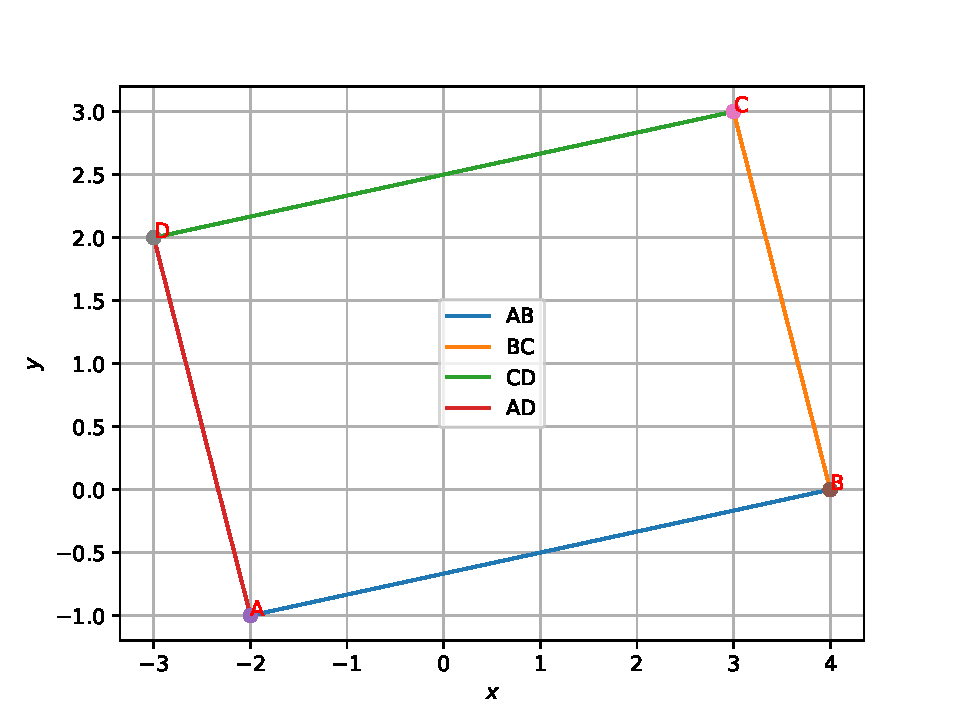
\includegraphics[width=\columnwidth]{./solutions/5/figs/quadrilateral/q4.eps}
	\caption{}
	\label{fig:2.2.5_qfour}	
	\end{figure}

%\section{\textbf{Question 3.1.5}}
%\subsection{Problem}

\renewcommand{\theequation}{\theenumi}
\begin{enumerate}[label=\thesection.\arabic*.,ref=\thesection.\theenumi]
\numberwithin{equation}{enumi}
	\item Two rails are represented as 
	\begin{multline}
	\myvec{1&2}\vec{x}=4\text{ and }\myvec{2&4}\vec{x}=12.
	\end{multline}
	\quad Will the rails cross each other?
	
	\solution The above equations can be represented as a matrix equation as
	\begin{align}\myvec{1&2\\2&4}\vec{x}=\myvec{4\\12}\vec{x}\end{align}
	The augmented matrix for the above matrix is row reduced as follows:
	\begin{align}\myvec{1&2&4\\2&4&12}\xleftrightarrow {R_2\leftarrow \frac{R_2}{2}}\myvec{1 & 2 & 4\\1 & 2 & 6} \\
\xleftrightarrow {R_2\leftarrow R_2 - R_1}\myvec{1 & 2 & 4\\0 & 0 & 2}
\end{align}
	Thus the row reduction of the 2$\times$3 matrix 
	\begin{align}
		\myvec{1&2&4\\2&4&12}
	\end{align}
	results in a matrix with two non zero rows having rank 2. Similarly the rank is 1 for the matrix$\myvec{1&2\\2&4}$\\
	As the rank of these two matrices aren't same, there is no solution. Therefore, the rails don't cross over eachother.
	The following python code computes the area of $\triangle$ABC in Fig.\ref{fig:qfive}.
	\begin{lstlisting}
	./codes/lines/q5.py
	\end{lstlisting}
	\begin{figure}[!ht]
	\centering
	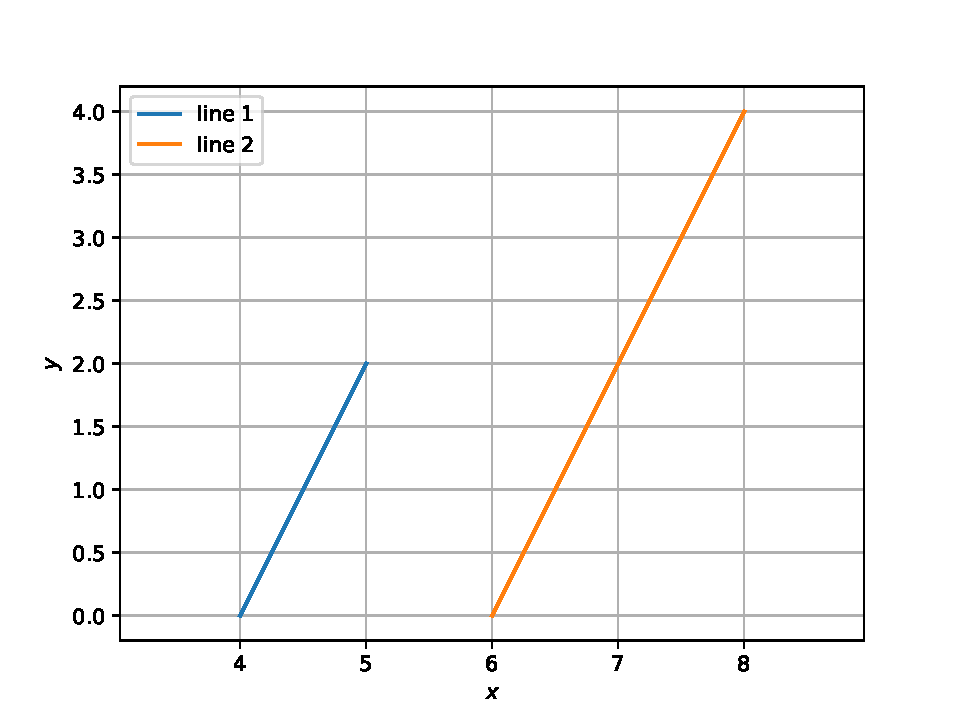
\includegraphics[width=\columnwidth]{./figs/lines/q5.pdf}
	\caption{Rails of Q.3.1.5}
	\label{fig:qfive}	
	\end{figure}
	
\end{enumerate}

\section{\textbf{Question 3.2.5}}
The following python code generates Fig. \ref{fig:3.11.5_qsix}.
	\begin{lstlisting}
	./solutions/5/codes/lines/q6.py
	\end{lstlisting}
	\begin{figure}[!ht]
	\centering
	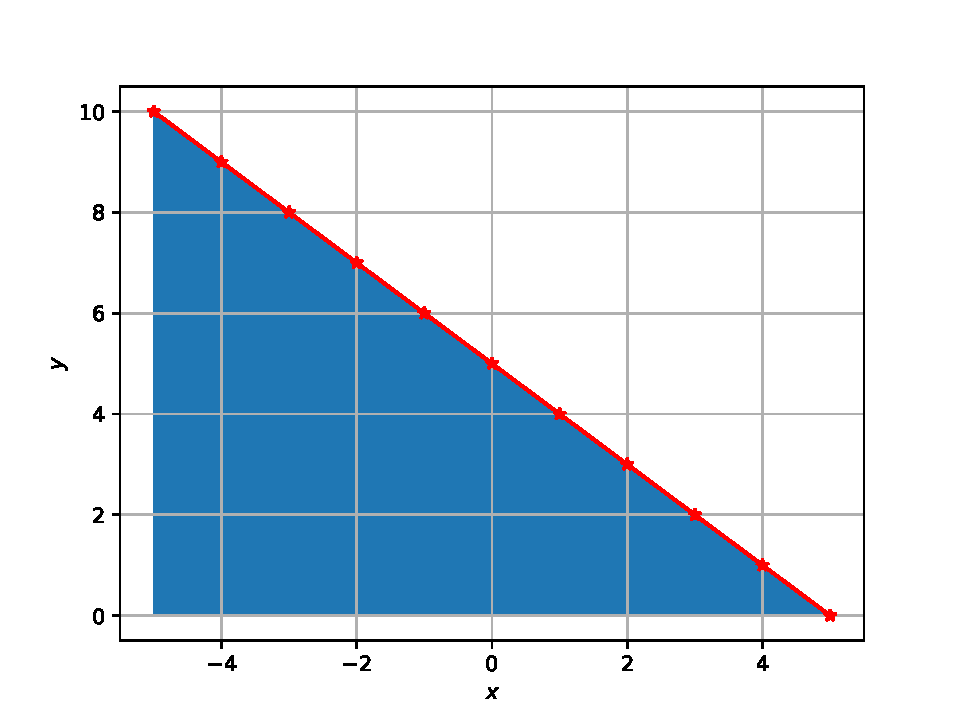
\includegraphics[width=\columnwidth]{./solutions/5/figs/lines/q6.eps}
	\caption{x+y$<$5}
	\label{fig:3.11.5_qsix}	
	\end{figure}
	

\section{\textbf{Question 3.3.5}}
 As the two matrices are equal their corresponding entries are also equal. Hence
\begin{align}
x+3&=0 \quad \implies x=-3
\\
z+4&=6 \quad \implies z=2
\\
2y-7&=3y-2 \quad \implies y=-5
\\
a-1&=-3 \quad \implies a=-2
\\
2c+2&=0 \quad \implies c=-1
\\
b-3&=2b+4 \quad \implies b=-7
\end{align}

\section{\textbf{Question 3.4.5}}
Using the polar form,
	\begin{align}
{\myvec{1\\\sqrt{3}}} = 2 \myvec{\cos 60\degree \\ \sin 60 \degree} &=2 \phase{60\degree}
\\
\implies 		\frac{-16}{\myvec{1\\\sqrt{3}}} = -8\phase{-60\degree} &= 4\myvec{-1 \\ \sqrt{3}}
	\end{align}
The following python code gives the desired answer
	\begin{lstlisting}
	./solutions/5/codes/lines/q8.py
	\end{lstlisting}

\section{\textbf{Question 3.5.5}}

	\begin{align}
\frac{ \brak{\vec{A}-\vec{B}}^T\myvec{1 \\ 0}}{\norm{\vec{A}-\vec{B}}\norm{\myvec{1 \\ 0}}} &= \frac{\myvec{-1 &1}^T\myvec{1 \\ 0}}{\norm{\myvec{-1 \\1}}\norm{\myvec{-1 \\1}}}
\\
&= -\frac{1}{\sqrt{2}} = \cos ^{-1}\brak{135\degree}
	\end{align}
Thus, the desired angle is $135\degree$.
	The following python code generates Fig. \ref{fig:3.5.5_qnine}.
	\begin{lstlisting}
	./solutions/5/codes/lines/q9.py
	\end{lstlisting}

	\begin{figure}[!ht]
	\centering
	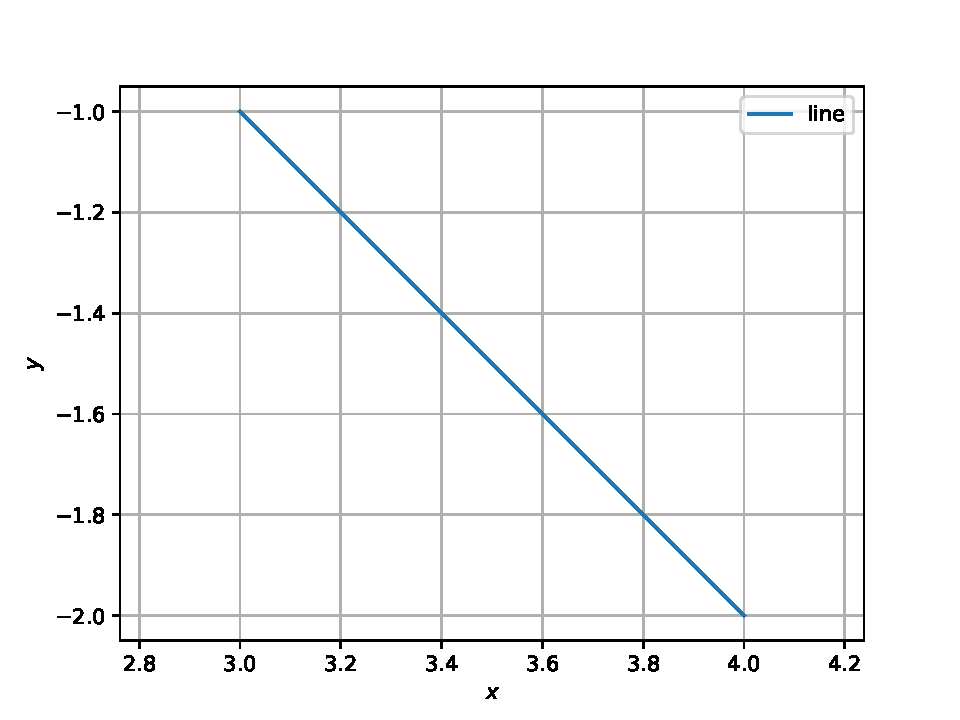
\includegraphics[width=\columnwidth]{./solutions/5/figs/lines/q9.eps}
	\caption{}
	\label{fig:3.5.5_qnine}	
	\end{figure}
	


\section{\textbf{Question 3.6.5}}
See Fig. \ref{fig:3.6.5_qten}.	In a parallelogram, the diagonals bisect each other. Hence
	\begin{align}
		\frac{\vec{A}+\vec{C}}{2} &= \frac{\vec{B}+\vec{D}}{2}
		\\
\therefore \frac{1+x}{2} = \frac{7}{2}, \frac{8}{2} &= \frac{y+5}{2} \\
\implies x=6,y&=3
\end{align}
	The following python code computes the value of x and y used in Fig. \ref{fig:3.6.5_qten}.
	\begin{lstlisting}
	./solutions/5/codes/lines/q10.py
	\end{lstlisting}
	\begin{figure}[!ht]
	\centering
	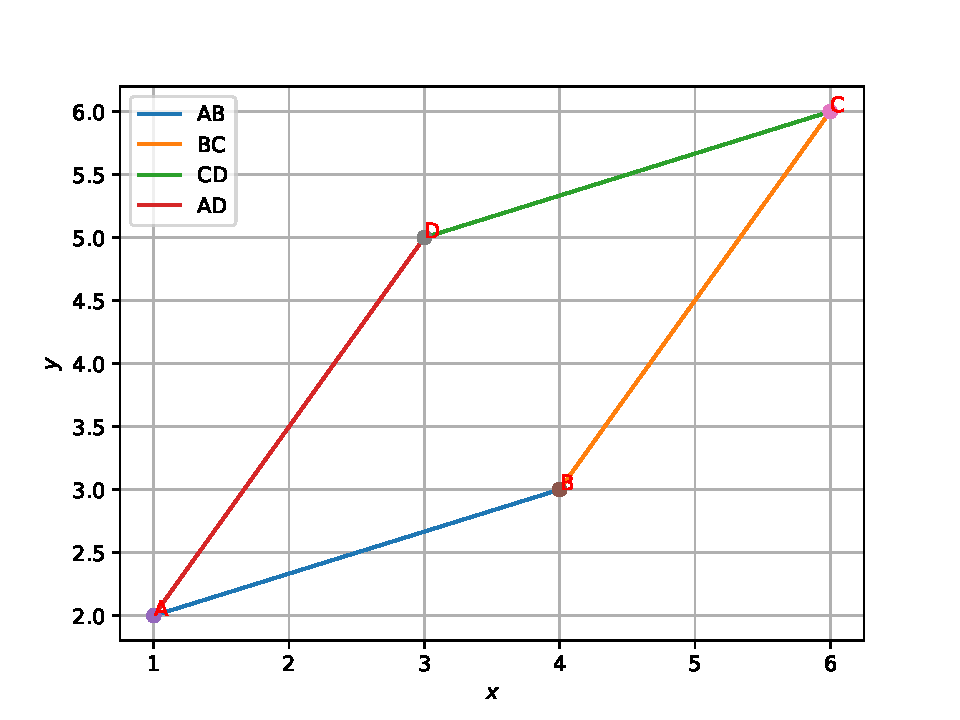
\includegraphics[width=\columnwidth]{./solutions/5/figs/lines/q10.eps}
	\caption{Parallelogram of Q.3.6.5}
	\label{fig:3.6.5_qten}	
	\end{figure}
	
		

\section{\textbf{Question 3.7.5}}
	The following python codes draw the graphs which are represented in Fig.\ref{fig:3.7.5_qelevena} and Fig.\ref{fig:3.7.5_qelevenb}.
	\begin{lstlisting}
	./solutions/5/codes/lines/q11a.py
	./solutions/5/codes/lines/q11b.py
	\end{lstlisting}
	\solution
	\begin{figure}[!ht]
	\centering
	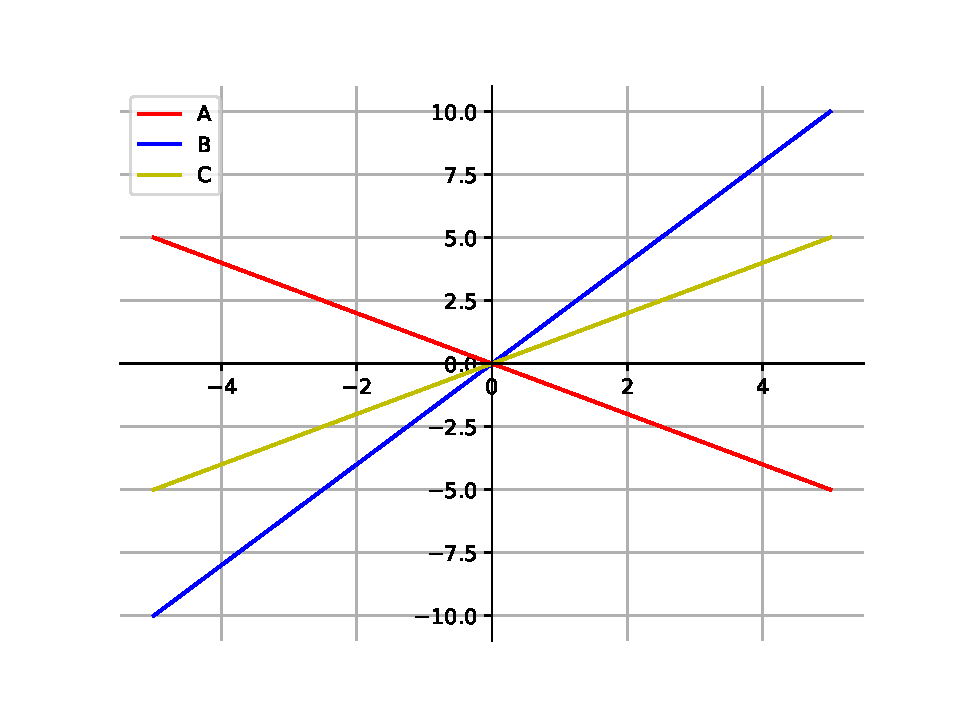
\includegraphics[width=\columnwidth]{./solutions/5/figs/lines/q11a.eps}
	\caption{}
	\label{fig:3.7.5_qelevena}	
	\end{figure}
	\begin{figure}[!ht]
	\centering
	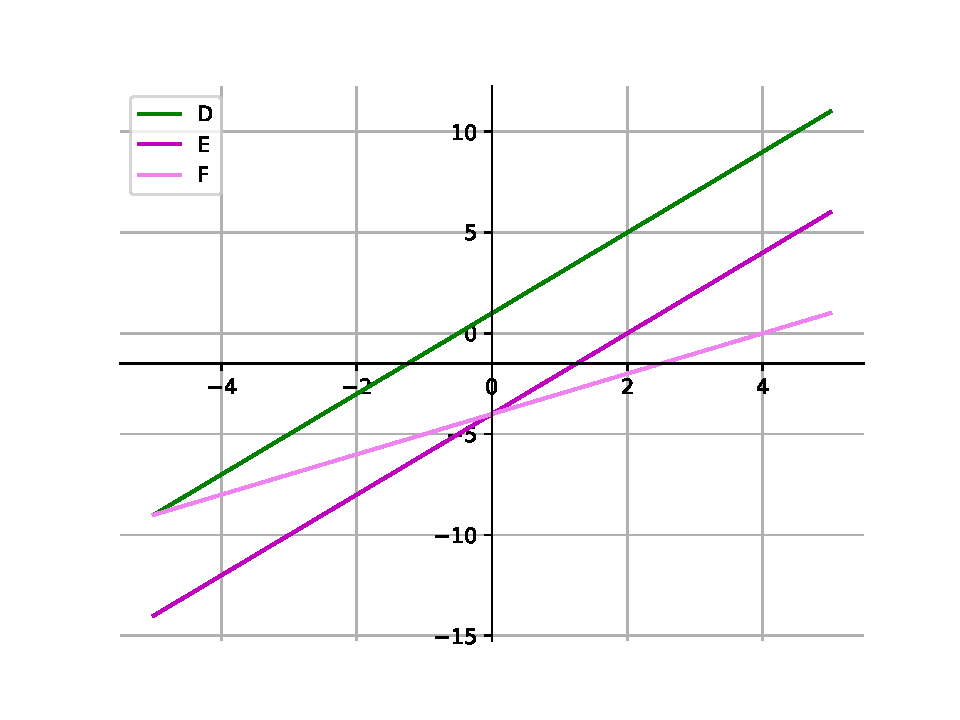
\includegraphics[width=\columnwidth]{./solutions/5/figs/lines/q11b.eps}
	\caption{}
	\label{fig:3.7.5_qelevenb}	
	\end{figure}
	

\section{\textbf{Question 3.8.5}}
See Fig. \ref{fig:3.8.5_qtwelve}.	
The velocity of rain and velocity of woman are
\begin{align}
\vec{v_r} &= \myvec{0\\-30}
\\
\vec{v_w} &= \myvec{-10\\0}
\end{align}
The relative velocity of rain w.r.t woman is given as
\begin{align}
\vec{v_{r_w}} &=\vec{v_r}- \vec{v_w}
\\
&=\myvec{10\\-30}
\end{align}
So the woman must hold the umbrella along the direction of $-\vec{v_{r_w}}$
Thus, the desired angle is 
\begin{align}
\theta={\tan}^{-1}\brak{\frac{10}{30}}
\end{align}
%
The following python code plots  Fig. \ref{fig:3.8.5_qtwelve}.
	\begin{lstlisting}
	./solutions/5/codes/lines/q12.py
	\end{lstlisting}
\begin{figure}[!ht]
	\centering
	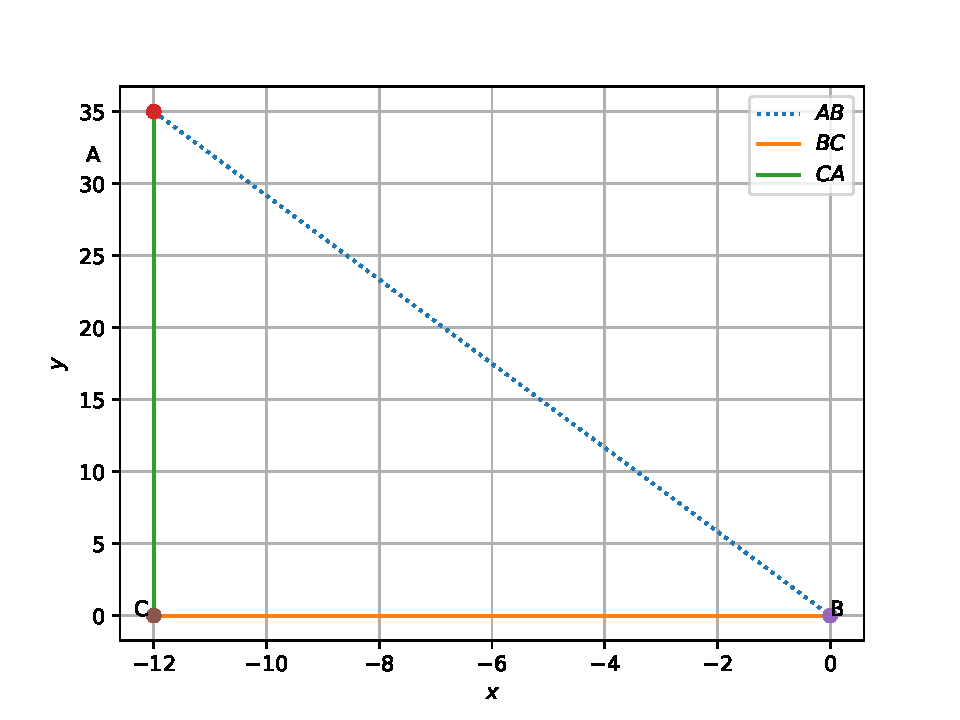
\includegraphics[width=\columnwidth]{./solutions/5/figs/lines/q12.eps}
	\caption{}
	\label{fig:3.8.5_qtwelve}	
	\end{figure}
	



\section{\textbf{Question 3.9.5}}
	
	The following python code computes the required matrix.
	\begin{lstlisting}
	./codes/lines/q13.py
	\end{lstlisting}
	
	\begin{enumerate}
		\item The matrix $A_{ij} = \frac{1}{2}|-3i+j|$ obtained is
		\begin{align}
			\myvec{0&0.5&1&1.5\\1.5&1&0.5&0\\3&2.5&2&1.5}
		\end{align}
		\item The matrix $A_{ij} = 2i-j$ obtained is
		\begin{align}
			\myvec{0&-1&-2&-3\\2&1&0&-1\\4&3&2&1}
		\end{align}
	\end{enumerate}
	
	

\section{\textbf{Question 3.10.5}}

The following python code computes the required determinant value.
	\begin{lstlisting}
	./solutions/5/codes/lines/q14.py
	\end{lstlisting}
	
	\begin{enumerate}
		\item $\mydet{3&-1&-2\\0&0&-1\\3&-5&0} = -12$
		\item $\mydet{3&-4&5\\1&1&-2\\2&3&1} = -46$
		\item $\mydet{0&1&2\\-1&0&-3\\-2&3&0}=0$
		\item $\mydet{2&-1&-2\\0&2&-1\\3&-5&0} = 5$

	\end{enumerate}

\section{\textbf{Question 3.11.5}}
	
Let x be an odd natural number and y be the odd natural number consecutive to x.
	\begin{align}
	\therefore y=x+2
	\end{align}
	We need to find x and y  such that 
	\begin{multline}
x,y >10 \text{ and } x+y<40\\
\therefore x+x+2<40\\
2x+2<40\\
x+1<20\\
x<19
	\end{multline}
	
	
	Hence the condition is satisfied when $x>10$ and $x<19$
	
	
	
	The following python code computes the required pairs of consecutive odd natural numbers which satisfy the required condition, shown in Fig.\ref{fig:3.11.5_fifteen}.
	\begin{lstlisting}
	./solutions/5/codes/lines/q15.py
	\end{lstlisting}
	\begin{figure}[!ht]
	\centering
	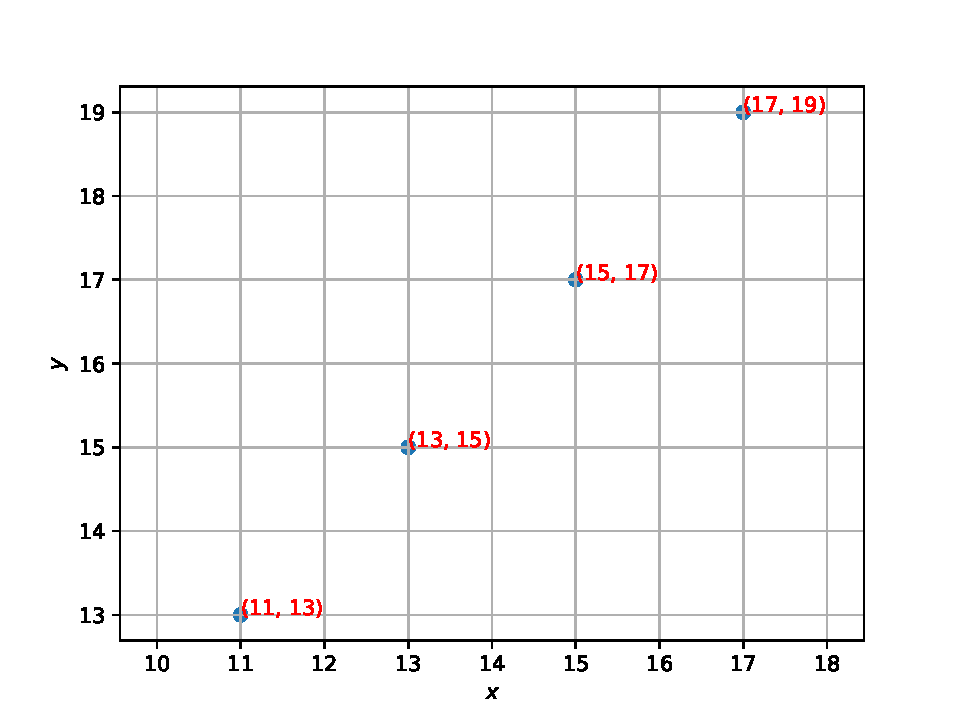
\includegraphics[width=\columnwidth]{./solutions/5/figs/lines/q15.eps}
	\caption{}
	\label{fig:3.11.5_fifteen}	
	\end{figure}

\section{\textbf{Question 3.12.5}}
	\begin{align}
		\norm{\vec{a}+\vec{b}}^2 &= \norm{\vec{a}}^2+2\vec{a}^T\vec{b}+\norm{\vec{b}}^2\\
&\le \norm{\vec{a}}^2+2\norm{\vec{a}}\norm{\vec{b}}+\norm{\vec{b}}^2\\
\implies 	\norm{\vec{a}+\vec{b}}^2 &\leq \brak{\norm{\vec{a}} + \norm{\vec{b}}}^2\\
\text{or, }		\norm{\vec{a}+\vec{b}} &\le  \norm{\vec{a}} + \norm{\vec{b}}
	\end{align}
using Cauchy-Schwarz inequality.

\section{\textbf{Question 4.1.5}}
	
From the Fig. \ref{fig:4.1.5_qseventeen} we obtain the coordinates as,
\begin{align}
\vec{O} = \myvec{0\\0} \quad\vec{A} = \myvec{0.707\\0.707} \quad\vec{B} = \myvec{0.707\\0} \quad\vec{C} = \myvec{1\\0} 
\end{align}
 The required area is the sector $OAC$.  This is given by
\begin{align}
ar\brak{OACB} &= ar\brak{OAB} + ar\brak{BAC}
\\
ar\brak{BAC} &= \frac{1}{2}\norm{\brak{\vec{B-A}}\times\brak{\vec{C-A}}}
\\
ar\brak{OAB} &= \frac{1}{2}\norm{\brak{\vec{B-O}}\times\brak{\vec{A-O}}}
\end{align}
which on computing, we obtain the required area as 0.3535
\begin{comment}
\begin{align}
\cos{\angle{BOA}} = \frac{\norm{\vec{OA}}^2 + \norm{\vec{OB}}^2 - \norm{\vec{AB}}^2}{2\norm{\vec{OA}}\norm{\vec{OB}}}
\\
\cos{\angle{BOA}} = \frac{1}{\sqrt{2}}
\\
\implies \angle{BOA} = 45\degree
\end{align}
 The required area is given by
\begin{align}
ar\brak{OACB} = \frac{\angle{BOA}}{360} \times \pi \times 1^2
\end{align}
\end{comment}
\begin{comment}
\begin{align} 
ar\brak{OACB} = ar\brak{OAB} + ar\brak{ACB}\\
ar\brak{OACB} = \int\limits_{0}^{0.707} x dx + \int\limits_{0.707}^{1} \sqrt{1-x^2}dx
\end{align}
\end{comment}

The following python code computes the required area represented in Fig.\ref{fig:4.1.5_qseventeen}.
	\begin{lstlisting}
	./solutions/5/codes/circle/q17ag.py
	\end{lstlisting}
\begin{figure}[!ht]
	\centering
	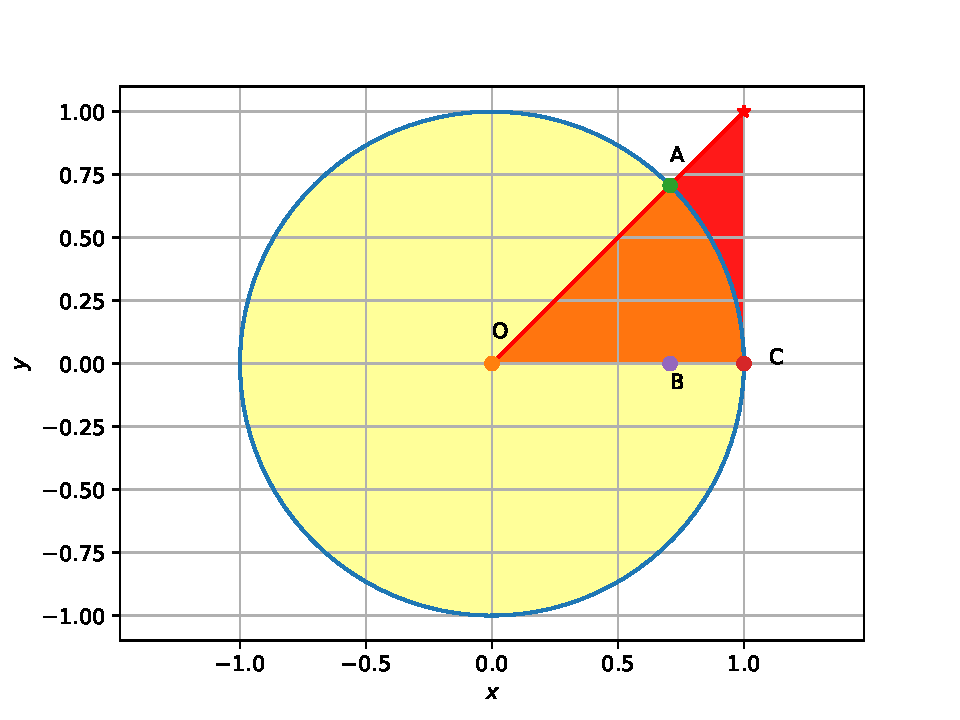
\includegraphics[width=\columnwidth]{./solutions/5/figs/circle/q17.eps}
	\caption{}
	\label{fig:4.1.5_qseventeen}	
	\end{figure}
	
\end{enumerate}

\section{\textbf{Question 4.2.5}}
The following python codes generate the required circle
	\begin{lstlisting}
	./solutions/5/codes/circle/q18abc.py
	./solutions/5/codes/circle/q18d.py
	\end{lstlisting}


\begin{enumerate}

\item \begin{align} 
\vec{x^Tx} - \myvec{4\\8}\vec{x} -45 = 0
\end{align}
See Fig. \ref{fig:4.2.5_qoeabc}.
\begin{align}
\vec{O} = \myvec{2\\4}, r = \sqrt{65} 
\end{align}
	\begin{figure}[!ht]
	\centering
	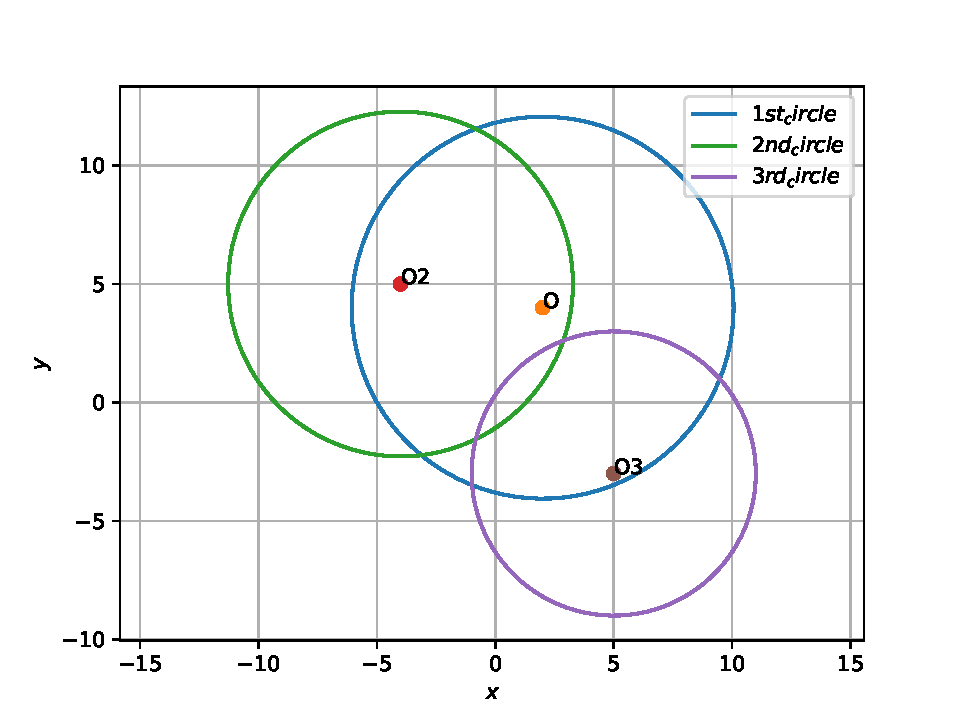
\includegraphics[width=\columnwidth]{./solutions/5/figs/circle/q18abc.eps}
	\caption{}
	\label{fig:4.2.5_qoeabc}	
	\end{figure}

\item See Fig. \ref{fig:4.2.5_qoeabc}.
\begin{align}
\vec{O} = \myvec{-4\\5}, r = \sqrt{53} 
\end{align}

\begin{align} 
\vec{x^Tx} - \myvec{8\\-10}\vec{x} - 12 = 0
\end{align}


\item See Fig. \ref{fig:4.2.5_qoeabc}.
\begin{align}
\vec{O} = \myvec{5\\-3}, r = 6
\end{align}
\begin{align} 
\norm{x - \myvec{5\\-3}} = 36
\end{align}



\begin{comment}
	\begin{figure}[!ht]
	\centering
	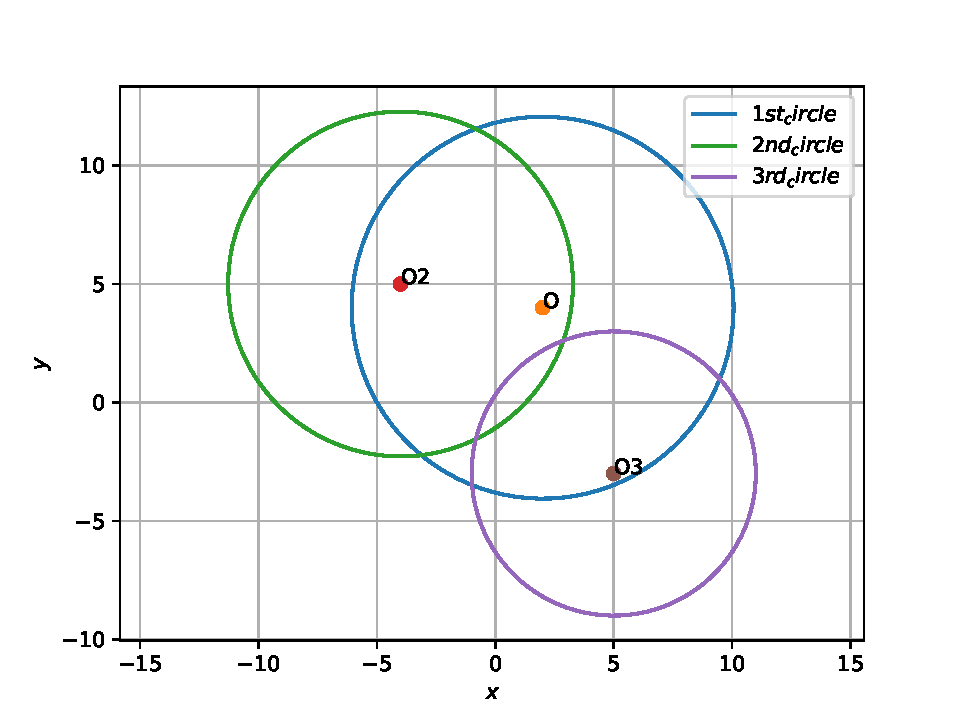
\includegraphics[width=\columnwidth]{./solutions/5/figs/circle/q18abc.eps}
	\caption{Circle of Q.4.2.5}
	\label{fig:4.2.5_qoeb}	
	\end{figure}
\end{comment}
\begin{comment}
	\begin{figure}[!ht]
	\centering
	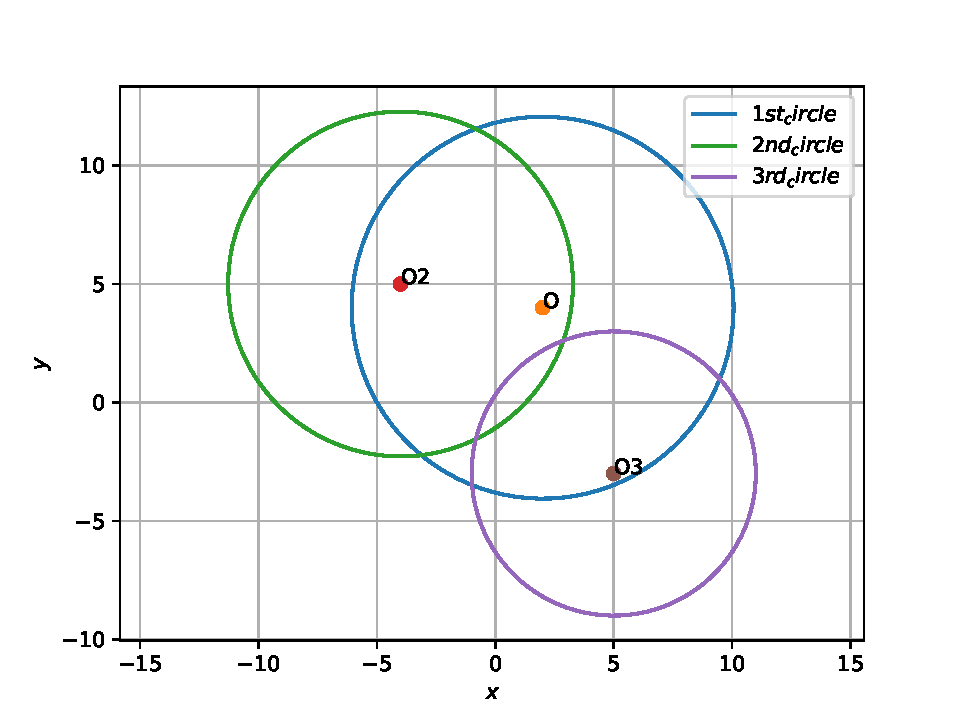
\includegraphics[width=\columnwidth]{./solutions/5/figs/circle/q18abc.eps}
	\caption{Circle of Q.4.2.5}
	\label{fig:4.2.5_qoec}	
	\end{figure}
\end{comment}
\item See Fig. \ref{fig:4.2.5_qoed}.
\begin{align}
\vec{O} = \frac{1}{4}\myvec{1\\0}, r = \frac{1}{4}
\end{align}
\begin{align} 
2\vec{x^Tx} - \myvec{1\\0}\vec{x} = 0
\end{align}
	\begin{figure}[!ht]
	\centering
	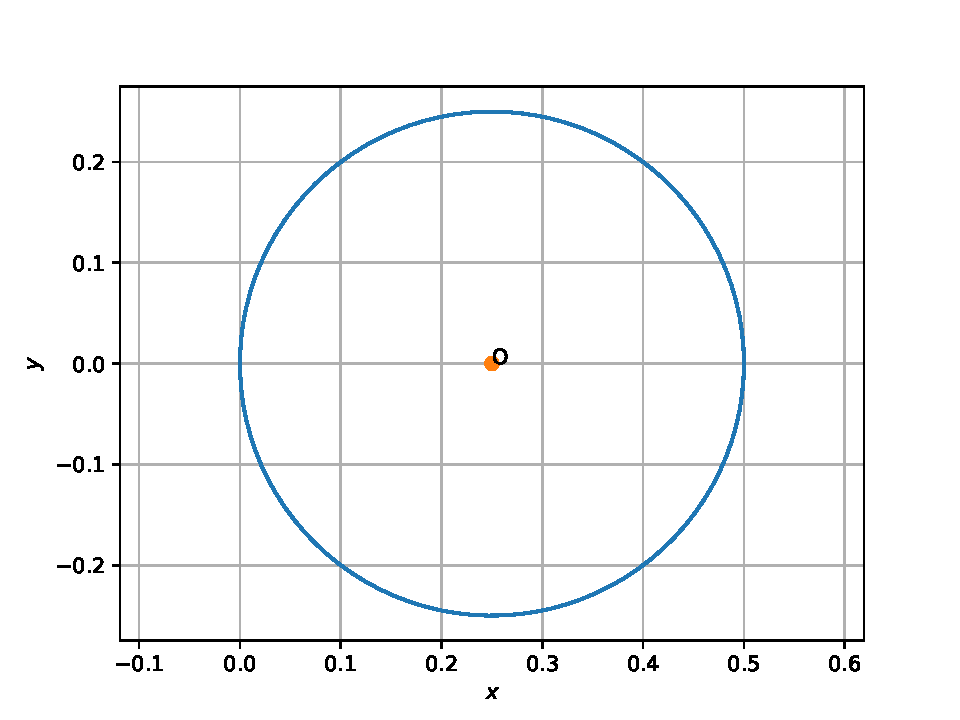
\includegraphics[width=\columnwidth]{./solutions/5/figs/circle/q18d.eps}
	\caption{}
	\label{fig:4.2.5_qoed}	
	\end{figure}



\end{enumerate}

\section{\textbf{Question 5.1.5}}
	
The vector form of 
\begin{align}
y = 6x^2-x-2 
\end{align}
is
\begin{align}
	\vec{x}^T\myvec{6&0\\0&0}\vec{x}  + \myvec{-1&-1}\vec{x} -2 = 0
	\end{align}
	Thus, 
	\begin{align}
	y = 0 \quad \implies 6x^2-x-2 &= 0
	\\
	\brak{x+\frac{1}{2}}\brak{x-\frac{2}{3}} &= 0
	\\
	x = \frac{-1}{2},\frac{2}{3}&
	\end{align}
	The following python code computes roots of the quadratic equation represented in Fig. \ref{fig:5.1.5_qnineteen}.
	\begin{lstlisting}
	./solutions/5/codes/conics/q19.py
	\end{lstlisting}
	\begin{figure}[!ht]
	\centering
	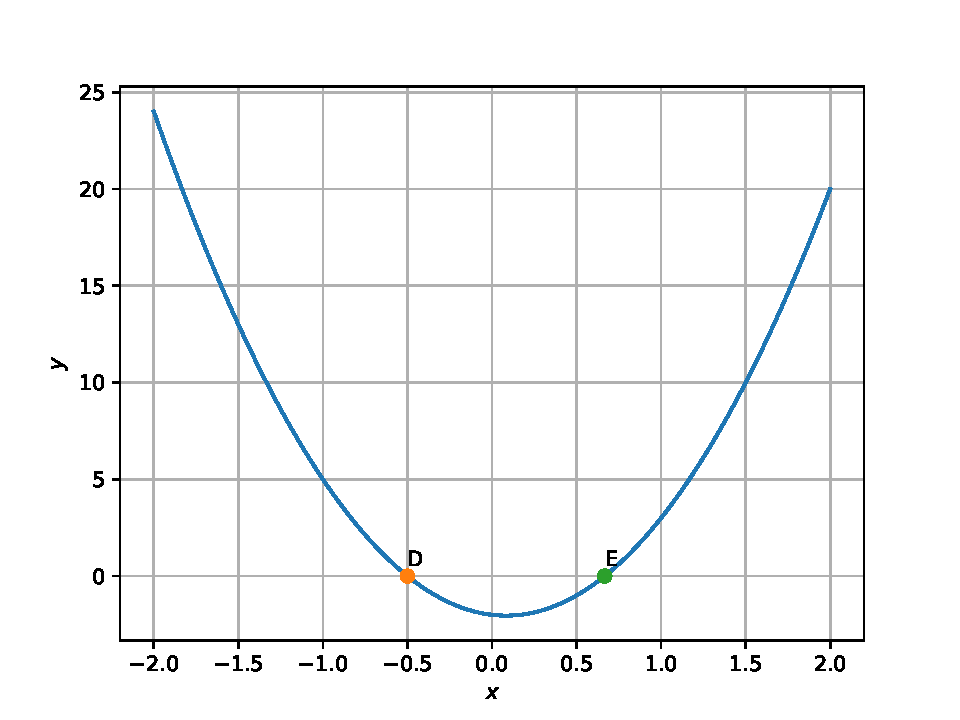
\includegraphics[width=\columnwidth]{./solutions/5/figs/conics/q19.eps}
	\caption{}
	\label{fig:5.1.5_qnineteen}	
	\end{figure}
	
	

\section{\textbf{Question 5.2.5}}
The following python code computes roots of the quadratic equation obtained:
	\begin{lstlisting}
	./solutions/5/codes/conics/q20a.py
	./solutions/5/codes/conics/q20b.py
	./solutions/5/codes/conics/q20c.py
	./solutions/5/codes/conics/q20d.py
	./solutions/5/codes/conics/q20e.py
	./solutions/5/codes/conics/q20f.py
	\end{lstlisting}
	
	\begin{enumerate}
	
		\item -1,$\frac{1}{4}$
	\begin{figure}[!ht]
	\centering
	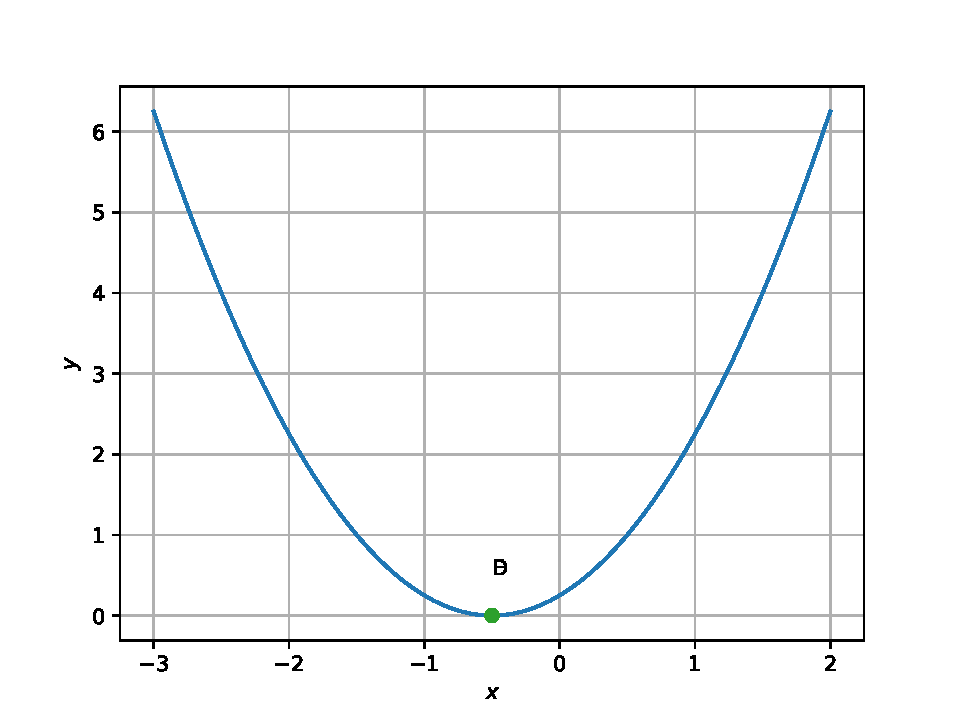
\includegraphics[width=\columnwidth]{./solutions/5/figs/conics/q20a.eps}
	\caption{}
	\label{fig:5.2.5_qtoa}	
	\end{figure}
	
		 For a general polynomial equation of degree 2,
	\begin{multline}
	p\brak{x,y} =
\\
 Ax^2 +Bxy + Cy^2 +Dx + Ey + F = 0\\
	\text{The vector form is}\\
	\vec{x}^T\myvec{A&\frac{B}{2}\\\frac{B}{2}&C}\vec{x}  + \myvec{D&E}\vec{x} + F = 0 \label{eq:5.2.5_qtwenty}
	\end{multline}
Here, sum of zeroes = D = -1\\
Product of zeroes = F =$\frac{1}{4}$\\
Substituing the values in \ref{eq:5.2.5_qtwenty},\\
\begin{multline}
\vec{x}^T\myvec{1&0\\0&0}\vec{x}  + 
\myvec{1&-1}\vec{x} +\frac{1}{4} = 0\\
\end{multline}
\begin{align}
\implies y = x^2 + x + \frac{1}{4}
\end{align}
The roots are -0.5 and -0.5 as represented in Fig. \ref{fig:5.2.5_qtoa}
		
		\item 1,1
	\begin{figure}[!ht]
	\centering
	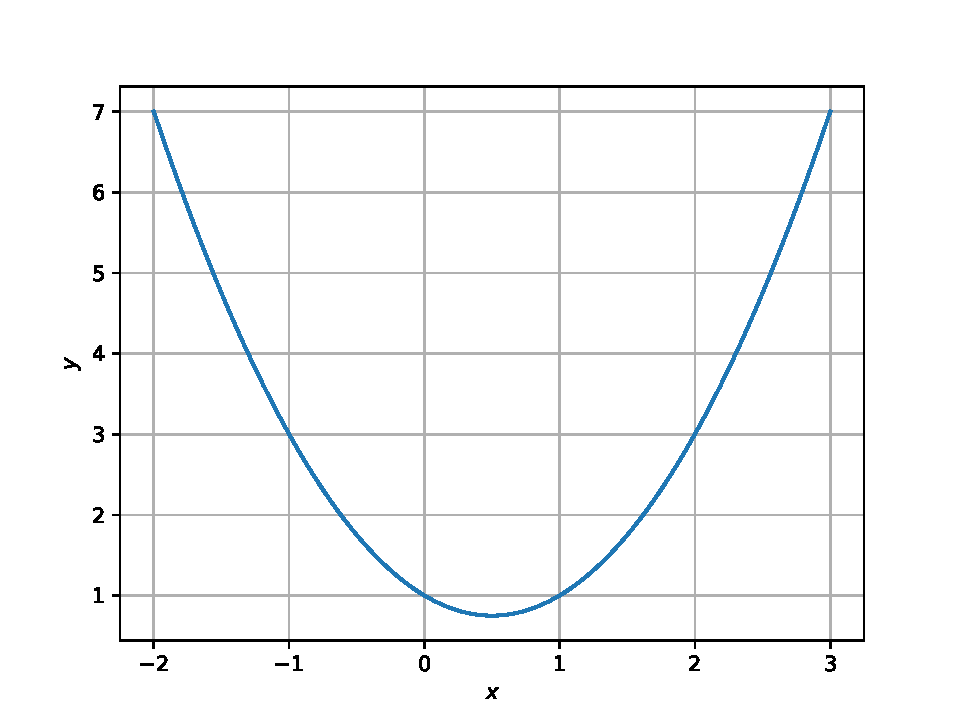
\includegraphics[width=\columnwidth]{./solutions/5/figs/conics/q20b.eps}
	\caption{}
	\label{fig:5.2.5_qtob}	
	\end{figure}
	
		
Here, sum of zeroes = D = 1\\
Product of zeroes = F =1\\
Substituing the values in \ref{eq:5.2.5_qtwenty},\\
\begin{multline}
\vec{x}^T\myvec{1&0\\0&0}\vec{x}  + \myvec{-1&-1}\vec{x} +1 = 0
\end{multline}
\begin{align}
\implies y = x^2 - x + 1 
\end{align}
Since the curve doesn't meet the x-axis, real roots don't exist for this parabola as represented in Fig. \ref{fig:5.2.5_qtob}	
		\item 0,$\sqrt{5}$
			\begin{figure}[!ht]
	\centering
	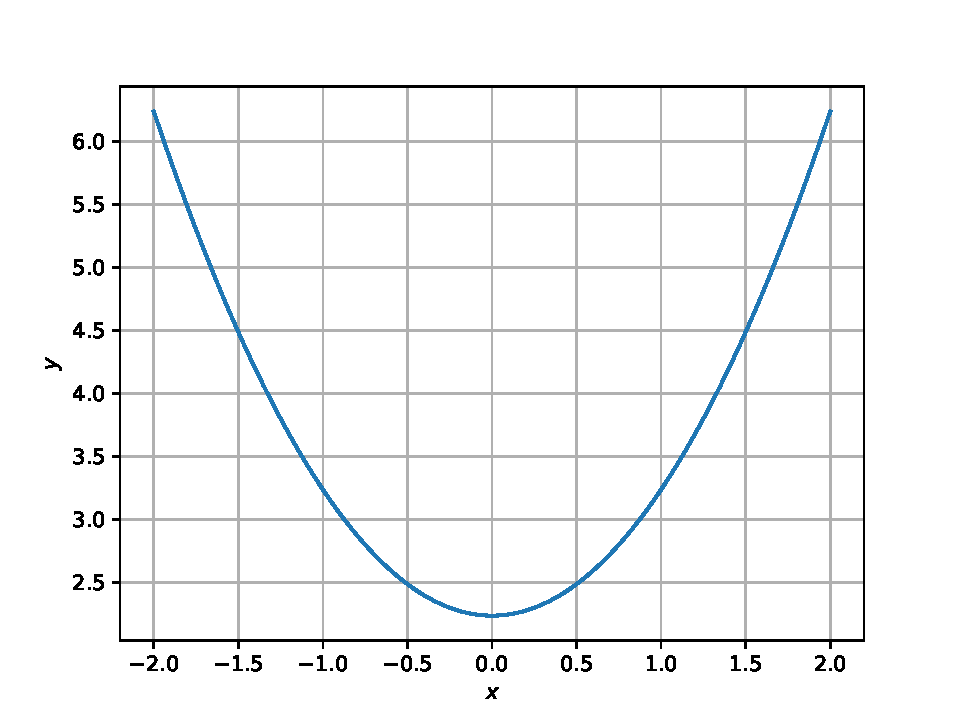
\includegraphics[width=\columnwidth]{./solutions/5/figs/conics/q20c.eps}
	\caption{}
	\label{fig:5.2.5_qtoc}	
	\end{figure}

		
Here, sum of zeroes = D = 0\\
Product of zeroes = F =$\sqrt{5}$\\
Substituing the values in \ref{eq:5.2.5_qtwenty},\\
\begin{multline}
\vec{x}^T\myvec{1&0\\0&0}\vec{x}  + \myvec{0&-1}\vec{x} + \sqrt{5} = 0
\end{multline}
\begin{align}
\implies y = x^2 + \sqrt{5}  
\end{align}
Since the curve doesn't meet the x-axis, real roots don't exist for this parabola as represented in Fig. \ref{fig:5.2.5_qtoc}	
		\item 4,1
	\begin{figure}[!ht]
	\centering
	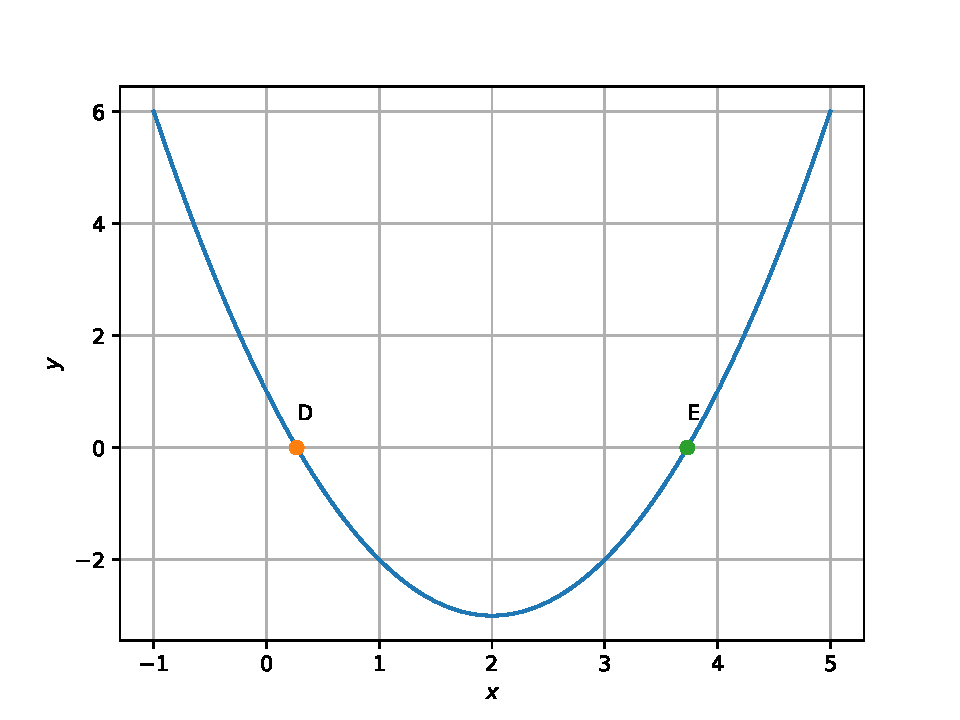
\includegraphics[width=\columnwidth]{./solutions/5/figs/conics/q20d.eps}
	\caption{}
	\label{fig:5.2.5_qtod}	
	\end{figure}
	
		 
Here, sum of zeroes = D = 4\\
Product of zeroes = F = 1\\
Substituing the values in \ref{eq:5.2.5_qtwenty},\\
\begin{multline}
\vec{x}^T\myvec{1&0\\0&0}\vec{x}  + \myvec{-4&-1}\vec{x} + 1 = 0
\end{multline}
\begin{align}
\implies y = x^2 - 4x + 1 
\end{align}
The roots are 3.73 and 0.26 as represented in Fig. \ref{fig:5.2.5_qtod}

		\item $\frac{1}{4}$,$\frac{1}{4}$
	\begin{figure}[!ht]
	\centering
	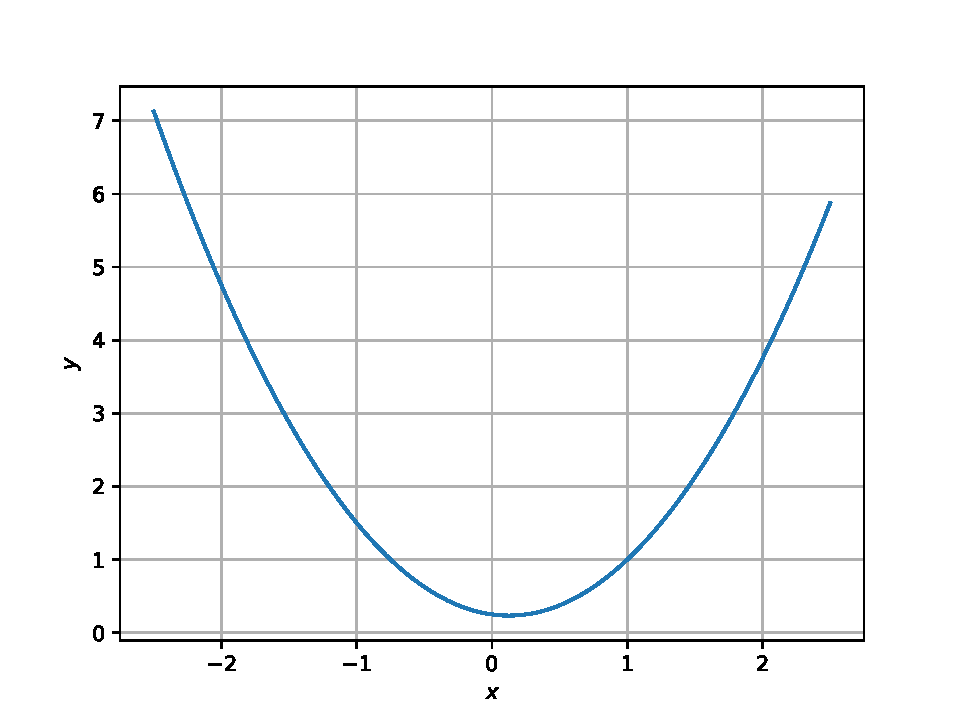
\includegraphics[width=\columnwidth]{./solutions/5/figs/conics/q20e.eps}
	\caption{}
	\label{fig:5.2.5_qtoe}	
	\end{figure}
		
 
Here, sum of zeroes = D = $\frac{1}{4}$\\
Product of zeroes = F = $\frac{1}{4}$\\
Substituing the values in \ref{eq:5.2.5_qtwenty},\\

\begin{multline}
\vec{x}^T\myvec{1&0\\0&0}\vec{x}  + \myvec{-\frac{1}{4}&-1}\vec{x} + \frac{1}{4} = 0
\end{multline}
\begin{align}
\implies y = x^2 - \frac{1}{4}x + \frac{1}{4} 
\end{align}
Since the curve doesn't meet the x-axis, real roots don't exist for this parabola as represented in Fig. \ref{fig:5.2.5_qtoe}	

		\item $\sqrt{2}$,$\frac{1}{3}$
	\begin{figure}[!ht]
	\centering
	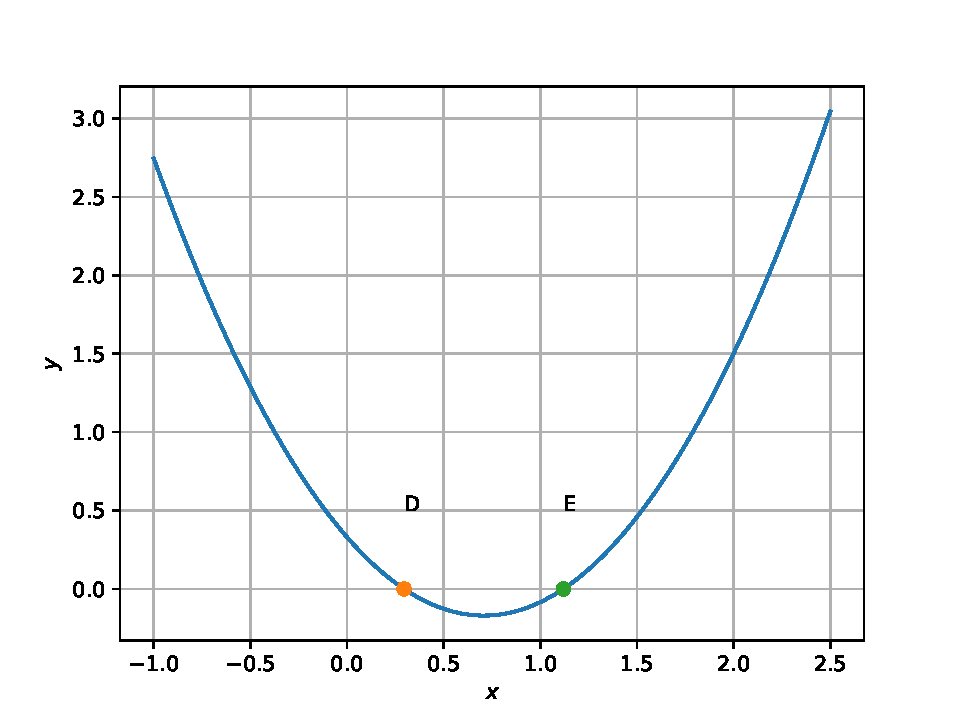
\includegraphics[width=\columnwidth]{./solutions/5/figs/conics/q20f.eps}
	\caption{}
	\label{fig:5.2.5_qtof}	
	\end{figure}

		

Here, sum of zeroes = D = $\sqrt{2}$\\
Product of zeroes = F = $\frac{1}{3}$\\
Substituing the values in \ref{eq:5.2.5_qtwenty},\\
\begin{multline}
\vec{x}^T\myvec{1&0\\0&0}\vec{x}  + \myvec{-\sqrt{2}&-1}\vec{x} + \frac{1}{3} = 0
\end{multline}
\begin{align}
\implies y = x^2 - \sqrt{2}x + \frac{1}{3}
\end{align}
The roots are 1.11 and 0.29 as represented in Fig. \ref{fig:5.2.5_qtof}
	\end{enumerate}

\end{document}
